\documentclass[11pt,a4paper]{article}

\usepackage[utf8]{inputenc}
\usepackage[T1]{fontenc}
\usepackage{tgpagella}
\usepackage[spanish]{babel}
\usepackage{geometry}
\usepackage{graphicx}
\usepackage{booktabs}
\usepackage{array}
\usepackage{xcolor}
\usepackage{titlesec}
\usepackage{fancyhdr}
\usepackage[parfill]{parskip}
\usepackage[expansion=false]{microtype}
\usepackage{hyperref}
\usepackage{setspace}
\usepackage{needspace}

\widowpenalty=10000
\clubpenalty=10000
\displaywidowpenalty=10000

\geometry{top=3.0cm,bottom=3.0cm,left=3.5cm,right=3.5cm}
\setlength{\parskip}{0.65em}
\setlength{\parindent}{0em}

\definecolor{azulai}{RGB}{30,80,140}
\definecolor{doradoai}{RGB}{140,90,0}
\definecolor{grisai}{RGB}{70,70,70}

\titleformat{\section}{\Large\bfseries\color{azulai}}{}{0em}{}[{\color{azulai}\titlerule[0.5pt]\nopagebreak[4]}]
\titlespacing*{\section}{0pt}{1.8em}{0.8em}

\titleformat{\subsection}{\large\bfseries\color{doradoai}}{}{0em}{}[{\nopagebreak[4]}]
\titlespacing*{\subsection}{0pt}{1.4em}{0.5em}

\titleformat{\subsubsection}{\normalsize\bfseries\color{grisai}}{}{0em}{}[{\nopagebreak[4]}]
\titlespacing*{\subsubsection}{0pt}{1.0em}{0.3em}

\pagestyle{fancy}\fancyhf{}
\rhead{\textcolor{grisai}{\small Izas — Arquitectura Interna}}
\lhead{\textcolor{grisai}{\small Figuras y configuraciones}}
\cfoot{\textcolor{grisai}{\small\thepage}}
\renewcommand{\headrulewidth}{0.3pt}

\hypersetup{colorlinks=true,linkcolor=azulai,urlcolor=azulai}
\setstretch{1.35}
\tolerance=1500
\emergencystretch=4em

\begin{document}

\begin{titlepage}
  \centering
  \vspace*{1.5cm}

  {\Huge\bfseries\color{azulai} Figuras y configuraciones}\\[0.5cm]
  {\large\color{grisai} Arquitectura Interna}\\[0.3cm]
  {\small\itshape\color{grisai} Arquitectura profunda de la carta natal}\\[2cm]

  {\huge\color{doradoai} Izas}\\[1.5cm]

  {\Large 16/04/1979 \quad 04:20}\\[0.3cm]
  {\Large Pamplona, España}\\[0.3cm]

  {\normalsize Lat: 42.8157° \quad Lon: -1.6522° \quad UTC+02:00}\\[0.3cm]

  {\normalsize Ascendente: Acuario 6°20' \quad
    MC: Escorpio 29°12'}\\[2cm]

  \vfill
  {\small Generado el 21/05/2026}
\end{titlepage}

\tableofcontents
\newpage

\section{Rueda natal}

\begin{figure}[h!]
  \centering
  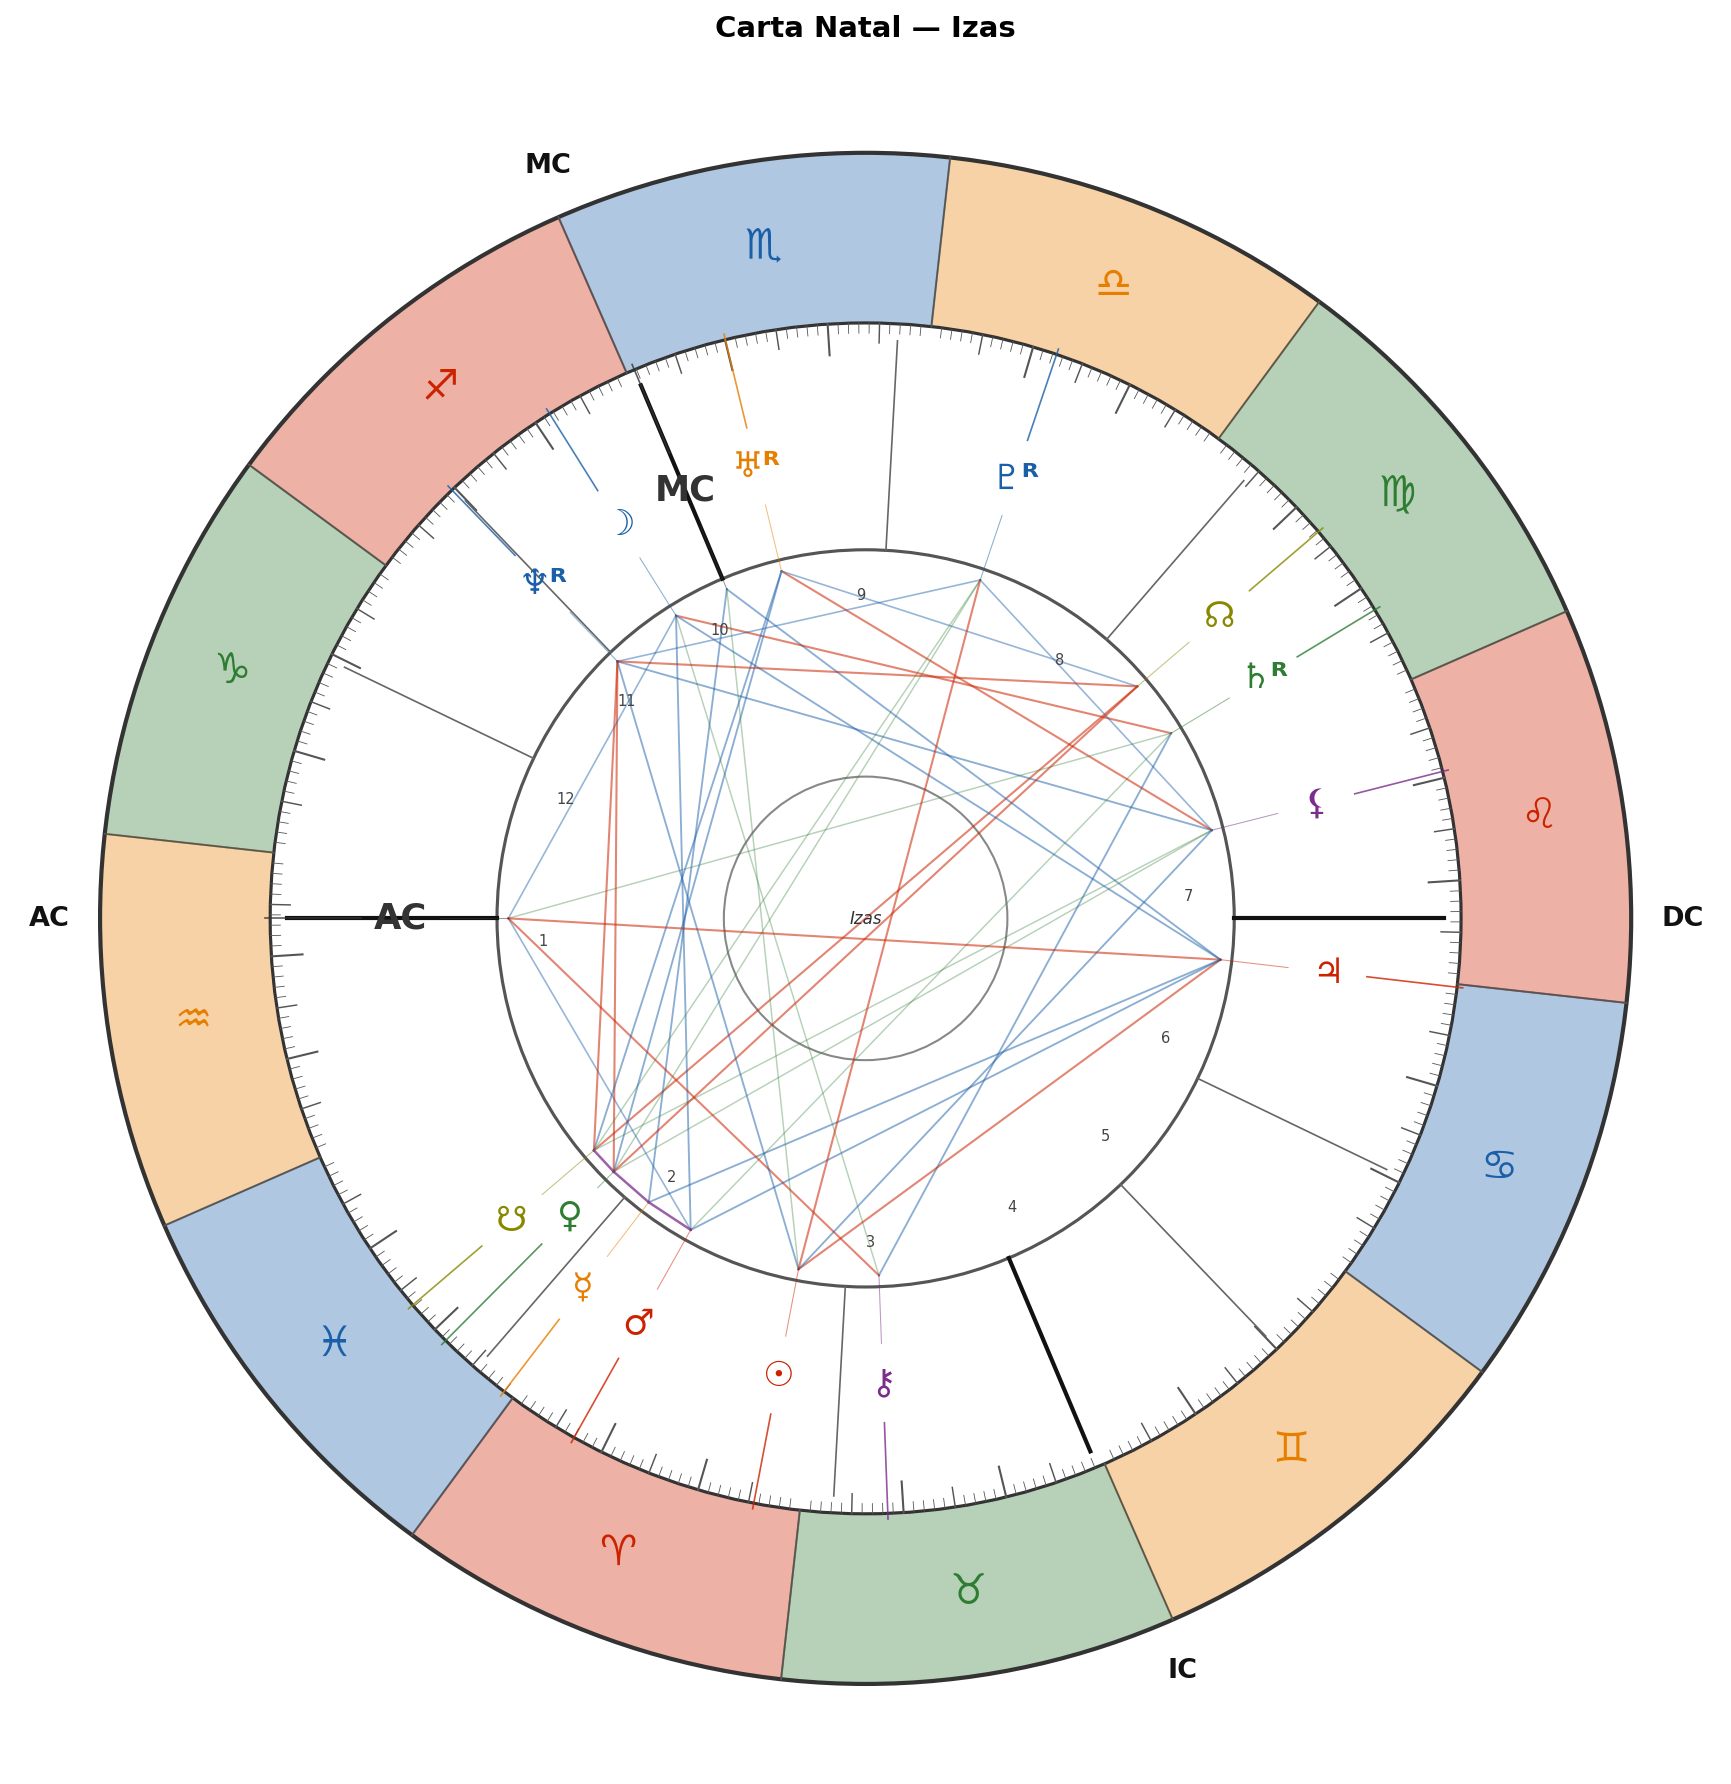
\includegraphics[width=0.90\textwidth]{Izas_Figuras_Configuraciones_rueda.png}
  \caption{Carta natal de Izas — 16/04/1979 04:20 — Pamplona, España}
\end{figure}

\newpage

\section{Puntos de referencia}

\begin{center}
\begin{tabular}{llrrll}
  \toprule
  \textbf{Punto} & \textbf{Signo} & \textbf{Grado} & \textbf{Casa} &
  \textbf{Elemento} & \textbf{R} \\
  \midrule
  Sol & Aries & 25°31' & 2 & Fuego &  \\
  Luna & Sagitario & 8°24' & 10 & Fuego &  \\
  Mercurio & Piscis & 28°57' & 2 & Agua &  \\
  Venus & Piscis & 21°30' & 1 & Agua &  \\
  Marte & Aries & 7°01' & 2 & Fuego &  \\
  Júpiter & Cáncer & 29°42' & 6 & Agua &  \\
  Saturno & Virgo & 7°33' & 7 & Tierra & R \\
  Urano & Escorpio & 19°58' & 9 & Agua & R \\
  Neptuno & Sagitario & 20°21' & 11 & Fuego & R \\
  Plutón & Libra & 17°38' & 8 & Aire & R \\
  Quirón & Tauro & 8°29' & 3 & Tierra &  \\
  Lilith & Leo & 20°38' & 7 & Fuego &  \\
  Nodo Norte & Virgo & 16°50' & 7 & Tierra &  \\
  Nodo Sur & Piscis & 16°50' & 1 & Agua &  \\
  Ascendente & Acuario & 6°20' & 1 & Aire &  \\
  Medio Cielo & Escorpio & 29°12' & 10 & Agua &  \\
  \bottomrule
\end{tabular}
\end{center}

\newpage

\section{Figuras detectadas}

\begin{center}
\begin{tabular}{p{3.2cm}p{7.2cm}p{2.8cm}r}
  \toprule
  \textbf{Figura} & \textbf{Puntos implicados} & \textbf{Casas} & \textbf{Peso} \\
  \midrule
  Cometa & Luna, Mercurio, Venus, Marte, Júpiter, Nodo Sur y Ascendente & Casas 1, 2, 6, 10 & 27 \\
  Cometa & Sol, Neptuno, Plutón y Lilith & Casas 2, 7, 8, 11 & 11 \\
  T-cuadrada & Mercurio, Venus, Marte, Neptuno, Nodo Norte y Nodo Sur & Casas 1, 2, 7, 11 & 18 \\
  Gran trígono & Mercurio, Venus, Marte, Júpiter, Nodo Sur y Medio Cielo & Casas 1, 2, 6, 10 & 22 \\
  Triángulo de aprendizaje & Luna, Mercurio, Venus, Marte, Saturno y Nodo Sur & Casas 1, 2, 7, 10 & 22 \\
  Triángulo de aprendizaje & Mercurio, Venus, Marte, Urano, Lilith y Nodo Sur & Casas 1, 2, 7, 9 & 18 \\
  Triángulo de aprendizaje & Mercurio, Venus, Marte, Neptuno, Lilith y Nodo Sur & Casas 1, 2, 7, 11 & 18 \\
  Triángulo de aprendizaje & Sol, Júpiter y Medio Cielo & Casas 2, 6, 10 & 13 \\
  Triángulo de aprendizaje & Luna, Saturno y Quirón & Casas 3, 7, 10 & 10 \\
  Triángulo de aprendizaje & Saturno, Quirón y Ascendente & Casas 1, 3, 7 & 10 \\
  Stellium & Mercurio, Venus, Marte y Nodo Sur & Casas 1, 2 & 14 \\
  Yod & Mercurio, Venus, Marte, Saturno, Nodo Sur y Ascendente & Casas 1, 2, 7 & 22 \\
  Yod & Mercurio, Venus, Marte, Plutón, Lilith y Nodo Sur & Casas 1, 2, 7, 8 & 18 \\
  \bottomrule
\end{tabular}
\end{center}

\vspace{0.8cm}

Las figuras muestran cómo varios puntos de la carta se conectan entre sí formando patrones mayores. No describen rasgos sueltos, sino modos completos de circulación interna: dónde se acumula tensión, dónde hay apoyo, qué zonas buscan salida y qué partes de la carta tienden a activarse juntas.

\newpage

\section{Interpretación de las configuraciones}

\subsection*{Dinámica central}
La carta no se organiza como una suma de figuras independientes. Hay configuraciones que funcionan como núcleo y otras que actúan como derivaciones, apoyos o zonas de ajuste.

Las configuraciones principales son: Cometa con Luna, Mercurio, Venus, Marte, Júpiter, Nodo Sur y Ascendente; T-cuadrada con Mercurio, Venus, Marte, Neptuno, Nodo Norte y Nodo Sur. Estas figuras marcan los grandes motores de la carta: dónde se concentra la tensión, dónde aparece dirección y qué zonas tienden a activarse juntas.

El stellium formado por Mercurio, Venus, Marte y Nodo Sur no debería leerse como una figura secundaria. Funciona como un núcleo de concentración desde el que se activan varias configuraciones. Por eso muchas figuras del documento no son procesos separados, sino distintas expresiones de ese mismo bloque interno.

La presencia de cometas indica que la carta no solo busca sostén: también necesita dirección. Hay recursos internos disponibles, pero la tensión de la oposición empuja a darles forma concreta.

La T-cuadrada principal muestra una presión que no puede resolverse solo desde comprensión mental. Necesita una forma de integración práctica: reconocer los dos polos, sostener la tensión y no descargarla siempre en el mismo punto.

Por eso, la lectura más importante no es cuántas figuras aparecen, sino qué estructura se repite: un núcleo concentrado, varios canales de sostén y una tensión que pide dirección consciente.

\subsection*{Configuraciones principales}

\Needspace{10\baselineskip}
\subsubsection*{Cometa — Luna, Mercurio, Venus, Marte, Júpiter, Nodo Sur y Ascendente}
Cometa: Luna, Mercurio, Venus, Marte, Júpiter, Nodo Sur y Ascendente. Se activa principalmente en Casas 1, 2, 6, 10.

La base de esta figura está formada por un gran trígono entre Luna, Mercurio, Venus, Marte, Júpiter y Nodo Sur. Ahí existe una circulación relativamente fluida de energía: recursos, capacidades y una forma bastante natural de sostener determinadas experiencias.

Sin embargo, la oposición entre Ascendente y Júpiter impide que esa energía quede cerrada sobre sí misma. La tensión empuja hacia movimiento, definición y dirección concreta.

El foco real de la figura está en Ascendente. Ahí suele concentrarse la necesidad de respuesta, visibilidad o transformación. Cuando esta energía no encuentra salida consciente, puede aparecer sensación de sobrecarga, exceso de presión interna o dificultad para dosificar.

La integración no pasa por eliminar la tensión, sino por usar el sostén del gran trígono como base para dirigir energía hacia algo concreto y vivo.

\Needspace{10\baselineskip}
\subsubsection*{T-cuadrada — Mercurio, Venus, Marte, Neptuno, Nodo Norte y Nodo Sur}
T-cuadrada: Mercurio, Venus, Marte, Neptuno, Nodo Norte y Nodo Sur. Se activa principalmente en Casas 1, 2, 7, 11.

La oposición entre Venus y Nodo Norte crea una polaridad interna importante. Las dos partes necesitan cosas distintas y rara vez se estabilizan del todo.

La energía de la figura descarga principalmente en Neptuno. Ahí suele aparecer la reacción, la sensación de presión o el intento de resolver rápidamente lo que se activa.

Esta configuración genera mucho movimiento interno. Puede dar capacidad de respuesta, resistencia y fuerza de transformación, pero también tendencia a vivir en exigencia constante o en sensación de urgencia.

La resolución no consiste en elegir uno de los polos y rechazar el otro. Consiste en construir suficiente estructura interna para sostener ambos sin reaccionar automáticamente.

\subsection*{Configuraciones de sostén y concentración}

\Needspace{10\baselineskip}
\subsubsection*{Gran trígono — Mercurio, Venus, Marte, Júpiter, Nodo Sur y Medio Cielo}
Gran trígono: Mercurio, Venus, Marte, Júpiter, Nodo Sur y Medio Cielo. Se activa principalmente en Casas 1, 2, 6, 10.

Esta figura crea un circuito de apoyo interno. La energía circula con relativa facilidad entre los puntos implicados, como si esas partes de la carta se reconocieran entre sí.

Puede funcionar como sostén, talento natural o capacidad espontánea de regulación. En momentos difíciles suele convertirse en una zona de apoyo importante.

El riesgo aparece cuando esta facilidad se convierte en circuito cerrado. La persona puede apoyarse siempre en la misma dinámica y evitar movimientos necesarios o situaciones que obliguen a salir de lo conocido.

La integración aparece cuando este sostén se usa como base para crecer, no como refugio permanente.

\Needspace{10\baselineskip}
\subsubsection*{Stellium — Mercurio, Venus, Marte y Nodo Sur}
Stellium: Mercurio, Venus, Marte y Nodo Sur. Se activa principalmente en Casas 1, 2.

Esta figura concentra mucha energía en Casa 1. No se activa una sola función psicológica: se moviliza un bloque entero de la carta.

Por eso este territorio puede sentirse especialmente intenso, absorbente o central en la vida. Ahí suele acumularse atención, presión, aprendizaje y necesidad de respuesta.

Cuando esta concentración no tiene suficiente regulación, puede aparecer saturación, exceso de identificación o dificultad para tomar distancia.

La integración pasa por aprender a dosificar la energía y evitar que toda la identidad quede atrapada dentro de un único territorio vital.

\subsection*{Figuras de ajuste}
Estas configuraciones no pesan tanto como estructura central, pero muestran zonas donde la carta necesita afinar respuestas, recolocar tensión o madurar patrones concretos.

\Needspace{8\baselineskip}
\subsubsection*{Cometa — Sol, Neptuno, Plutón y Lilith}
Cometa: Sol, Neptuno, Plutón y Lilith. Se activa principalmente en Casas 2, 7, 8, 11.

La base de esta figura está formada por un gran trígono entre Sol, Neptuno y Lilith. Ahí existe una circulación relativamente fluida de energía: recursos, capacidades y una forma bastante natural de sostener determinadas experiencias.

Sin embargo, la oposición entre Plutón y Sol impide que esa energía quede cerrada sobre sí misma. La tensión empuja hacia movimiento, definición y dirección concreta.

El foco real de la figura está en Plutón. Ahí suele concentrarse la necesidad de respuesta, visibilidad o transformación. Cuando esta energía no encuentra salida consciente, puede aparecer sensación de sobrecarga, exceso de presión interna o dificultad para dosificar.

La integración no pasa por eliminar la tensión, sino por usar el sostén del gran trígono como base para dirigir energía hacia algo concreto y vivo.

\Needspace{8\baselineskip}
\subsubsection*{Triángulo de aprendizaje — Luna, Mercurio, Venus, Marte, Saturno y Nodo Sur}
Triángulo de aprendizaje: Luna, Mercurio, Venus, Marte, Saturno y Nodo Sur. Se activa principalmente en Casas 1, 2, 7, 10.

La tensión principal aparece en la cuadratura entre Luna y Saturno. Ahí suele haber fricción, exigencia o sensación de incompatibilidad entre dos formas de responder.

El quincuncio entre Marte y Saturno obliga a reajustar constantemente la respuesta. No se resuelve desde control directo, sino desde observación fina y capacidad de adaptación.

El trígono entre Luna y Marte funciona como apoyo interno. Ahí existe una posibilidad de sostén, comprensión o regulación que ayuda a integrar la figura.

Este tipo de configuración suele madurar lentamente. No se resuelve de una vez: se afina con experiencia, repetición y capacidad de reconocer cuándo estás reaccionando desde automatismo.

\Needspace{8\baselineskip}
\subsubsection*{Triángulo de aprendizaje — Mercurio, Venus, Marte, Urano, Lilith y Nodo Sur}
Triángulo de aprendizaje: Mercurio, Venus, Marte, Urano, Lilith y Nodo Sur. Se activa principalmente en Casas 1, 2, 7, 9.

La tensión principal aparece en la cuadratura entre Urano y Lilith. Ahí suele haber fricción, exigencia o sensación de incompatibilidad entre dos formas de responder.

El quincuncio entre Venus y Lilith obliga a reajustar constantemente la respuesta. No se resuelve desde control directo, sino desde observación fina y capacidad de adaptación.

El trígono entre Venus y Urano funciona como apoyo interno. Ahí existe una posibilidad de sostén, comprensión o regulación que ayuda a integrar la figura.

Este tipo de configuración suele madurar lentamente. No se resuelve de una vez: se afina con experiencia, repetición y capacidad de reconocer cuándo estás reaccionando desde automatismo.

\Needspace{8\baselineskip}
\subsubsection*{Triángulo de aprendizaje — Mercurio, Venus, Marte, Neptuno, Lilith y Nodo Sur}
Triángulo de aprendizaje: Mercurio, Venus, Marte, Neptuno, Lilith y Nodo Sur. Se activa principalmente en Casas 1, 2, 7, 11.

La tensión principal aparece en la cuadratura entre Venus y Neptuno. Ahí suele haber fricción, exigencia o sensación de incompatibilidad entre dos formas de responder.

El quincuncio entre Venus y Lilith obliga a reajustar constantemente la respuesta. No se resuelve desde control directo, sino desde observación fina y capacidad de adaptación.

El trígono entre Neptuno y Lilith funciona como apoyo interno. Ahí existe una posibilidad de sostén, comprensión o regulación que ayuda a integrar la figura.

Este tipo de configuración suele madurar lentamente. No se resuelve de una vez: se afina con experiencia, repetición y capacidad de reconocer cuándo estás reaccionando desde automatismo.

\Needspace{8\baselineskip}
\subsubsection*{Triángulo de aprendizaje — Sol, Júpiter y Medio Cielo}
Triángulo de aprendizaje: Sol, Júpiter y Medio Cielo. Se activa principalmente en Casas 2, 6, 10.

La tensión principal aparece en la cuadratura entre Sol y Júpiter. Ahí suele haber fricción, exigencia o sensación de incompatibilidad entre dos formas de responder.

El quincuncio entre Sol y Medio Cielo obliga a reajustar constantemente la respuesta. No se resuelve desde control directo, sino desde observación fina y capacidad de adaptación.

El trígono entre Júpiter y Medio Cielo funciona como apoyo interno. Ahí existe una posibilidad de sostén, comprensión o regulación que ayuda a integrar la figura.

Este tipo de configuración suele madurar lentamente. No se resuelve de una vez: se afina con experiencia, repetición y capacidad de reconocer cuándo estás reaccionando desde automatismo.

\Needspace{8\baselineskip}
\subsubsection*{Triángulo de aprendizaje — Luna, Saturno y Quirón}
Triángulo de aprendizaje: Luna, Saturno y Quirón. Se activa principalmente en Casas 3, 7, 10.

La tensión principal aparece en la cuadratura entre Luna y Saturno. Ahí suele haber fricción, exigencia o sensación de incompatibilidad entre dos formas de responder.

El quincuncio entre Luna y Quirón obliga a reajustar constantemente la respuesta. No se resuelve desde control directo, sino desde observación fina y capacidad de adaptación.

El trígono entre Saturno y Quirón funciona como apoyo interno. Ahí existe una posibilidad de sostén, comprensión o regulación que ayuda a integrar la figura.

Este tipo de configuración suele madurar lentamente. No se resuelve de una vez: se afina con experiencia, repetición y capacidad de reconocer cuándo estás reaccionando desde automatismo.

\Needspace{8\baselineskip}
\subsubsection*{Triángulo de aprendizaje — Saturno, Quirón y Ascendente}
Triángulo de aprendizaje: Saturno, Quirón y Ascendente. Se activa principalmente en Casas 1, 3, 7.

La tensión principal aparece en la cuadratura entre Quirón y Ascendente. Ahí suele haber fricción, exigencia o sensación de incompatibilidad entre dos formas de responder.

El quincuncio entre Saturno y Ascendente obliga a reajustar constantemente la respuesta. No se resuelve desde control directo, sino desde observación fina y capacidad de adaptación.

El trígono entre Saturno y Quirón funciona como apoyo interno. Ahí existe una posibilidad de sostén, comprensión o regulación que ayuda a integrar la figura.

Este tipo de configuración suele madurar lentamente. No se resuelve de una vez: se afina con experiencia, repetición y capacidad de reconocer cuándo estás reaccionando desde automatismo.

\Needspace{8\baselineskip}
\subsubsection*{Yod — Mercurio, Venus, Marte, Saturno, Nodo Sur y Ascendente}
Yod: Mercurio, Venus, Marte, Saturno, Nodo Sur y Ascendente. Se activa principalmente en Casas 1, 2, 7.

La base formada entre Marte y Ascendente crea una posibilidad de apoyo o compensación relativamente estable.

Sin embargo, toda la figura apunta hacia Saturno. Ahí aparece una presión difícil de controlar racionalmente, como si una parte de la carta necesitara reajustarse continuamente.

El Yod no suele sentirse como conflicto frontal. Opera más bien como una incomodidad persistente, una sensación de que algo necesita recolocarse aunque no siempre resulte fácil entender exactamente qué.

La integración llega cuando dejas de intentar forzar respuestas inmediatas y empiezas a trabajar con más precisión, escucha y capacidad de ajuste.

\Needspace{8\baselineskip}
\subsubsection*{Yod — Mercurio, Venus, Marte, Plutón, Lilith y Nodo Sur}
Yod: Mercurio, Venus, Marte, Plutón, Lilith y Nodo Sur. Se activa principalmente en Casas 1, 2, 7, 8.

La base formada entre Plutón y Lilith crea una posibilidad de apoyo o compensación relativamente estable.

Sin embargo, toda la figura apunta hacia Venus. Ahí aparece una presión difícil de controlar racionalmente, como si una parte de la carta necesitara reajustarse continuamente.

El Yod no suele sentirse como conflicto frontal. Opera más bien como una incomodidad persistente, una sensación de que algo necesita recolocarse aunque no siempre resulte fácil entender exactamente qué.

La integración llega cuando dejas de intentar forzar respuestas inmediatas y empiezas a trabajar con más precisión, escucha y capacidad de ajuste.



\Needspace{10\baselineskip}
\section{Integración}

\vspace{1cm}

\begin{center}
{\small\itshape\color{grisai}
La astrología se usa aquí como lenguaje simbólico de observación, no como una definición cerrada de la persona.\\
Este documento muestra patrones de organización interna, no un destino fijo.
}
\end{center}

\end{document}
